\section{Results}\label{sec:results}
\subsection{Proving and Verifying Times}\label{subsec:results:provingverifying}

\begin{figure*}[!htb]
    \centering
    \subfloat[\centering Proving Time]{{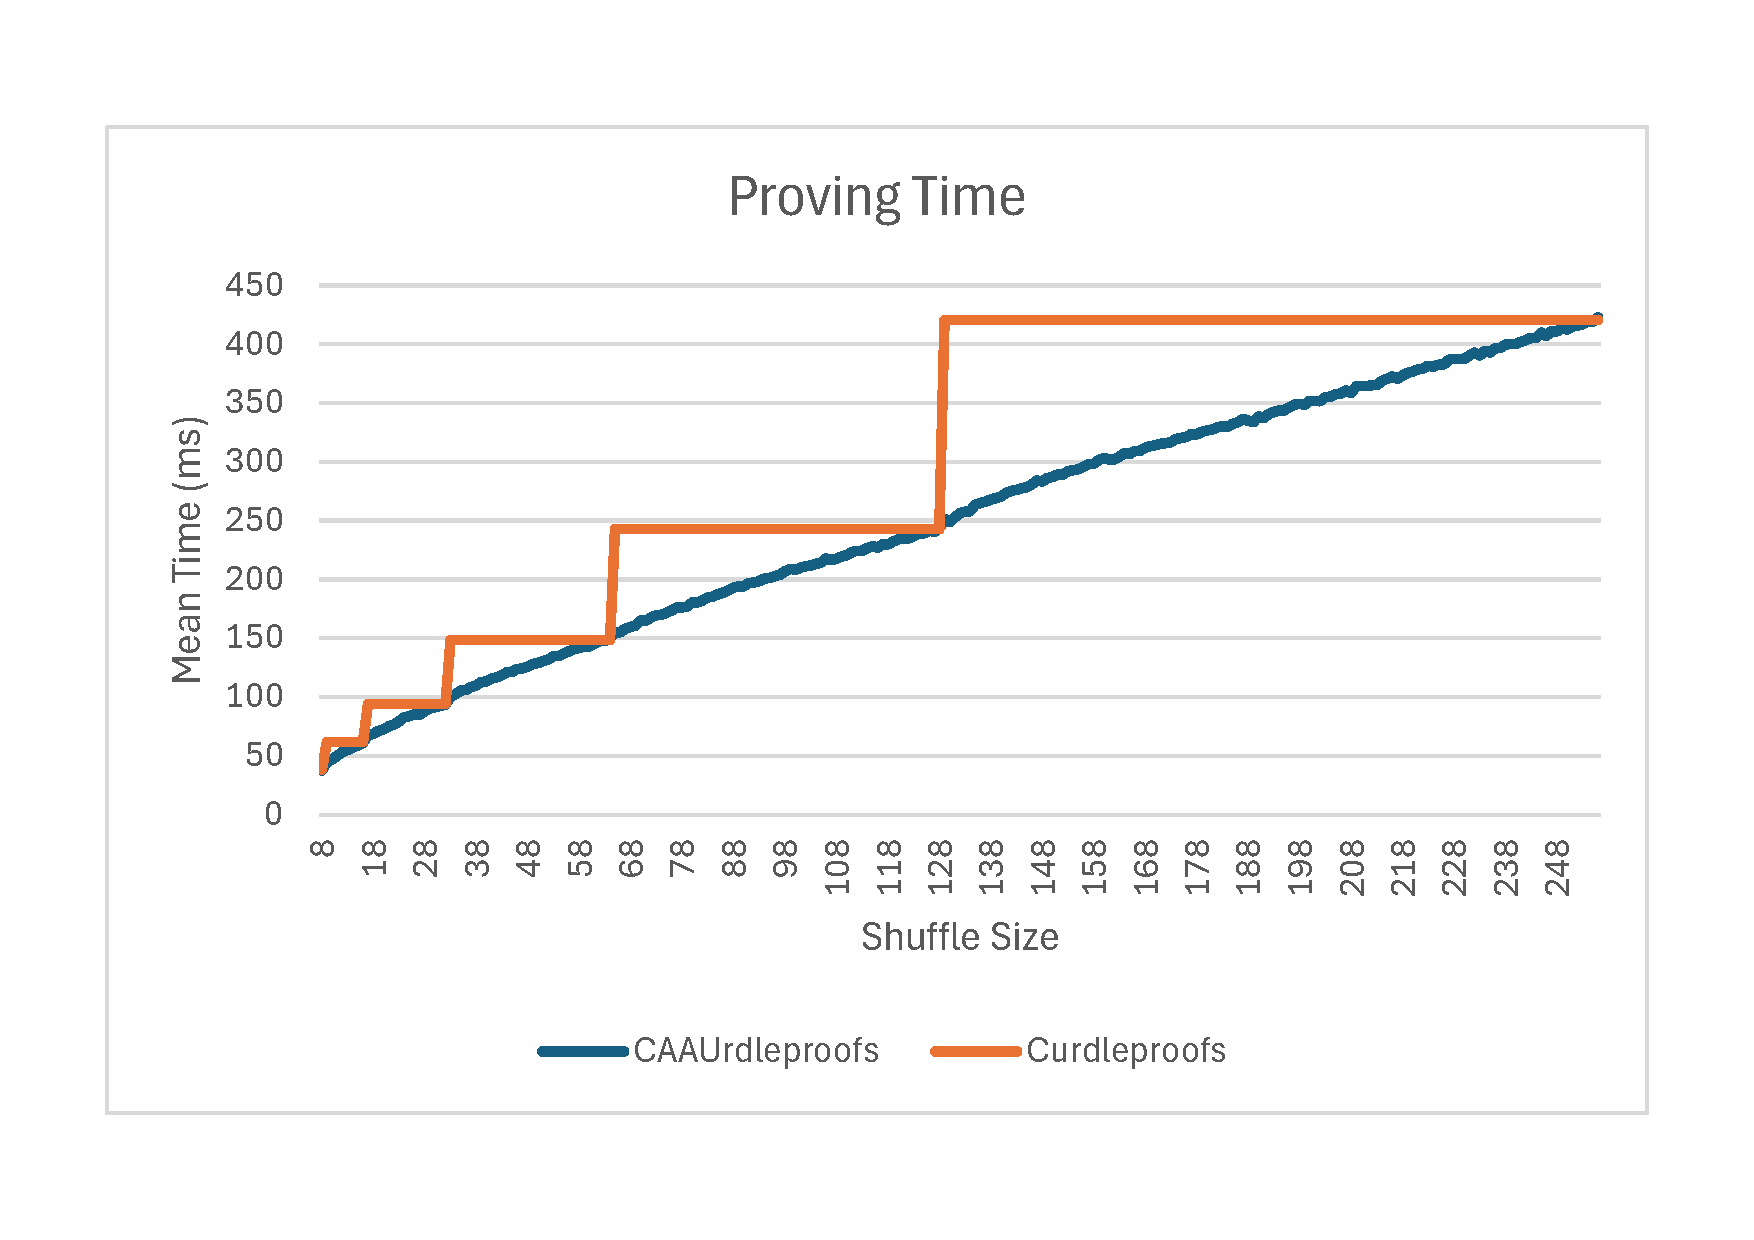
\includegraphics[width=0.45\textwidth]{figures/results/provingtime} }}%
    \qquad
    \subfloat[\centering Verifying Time]{{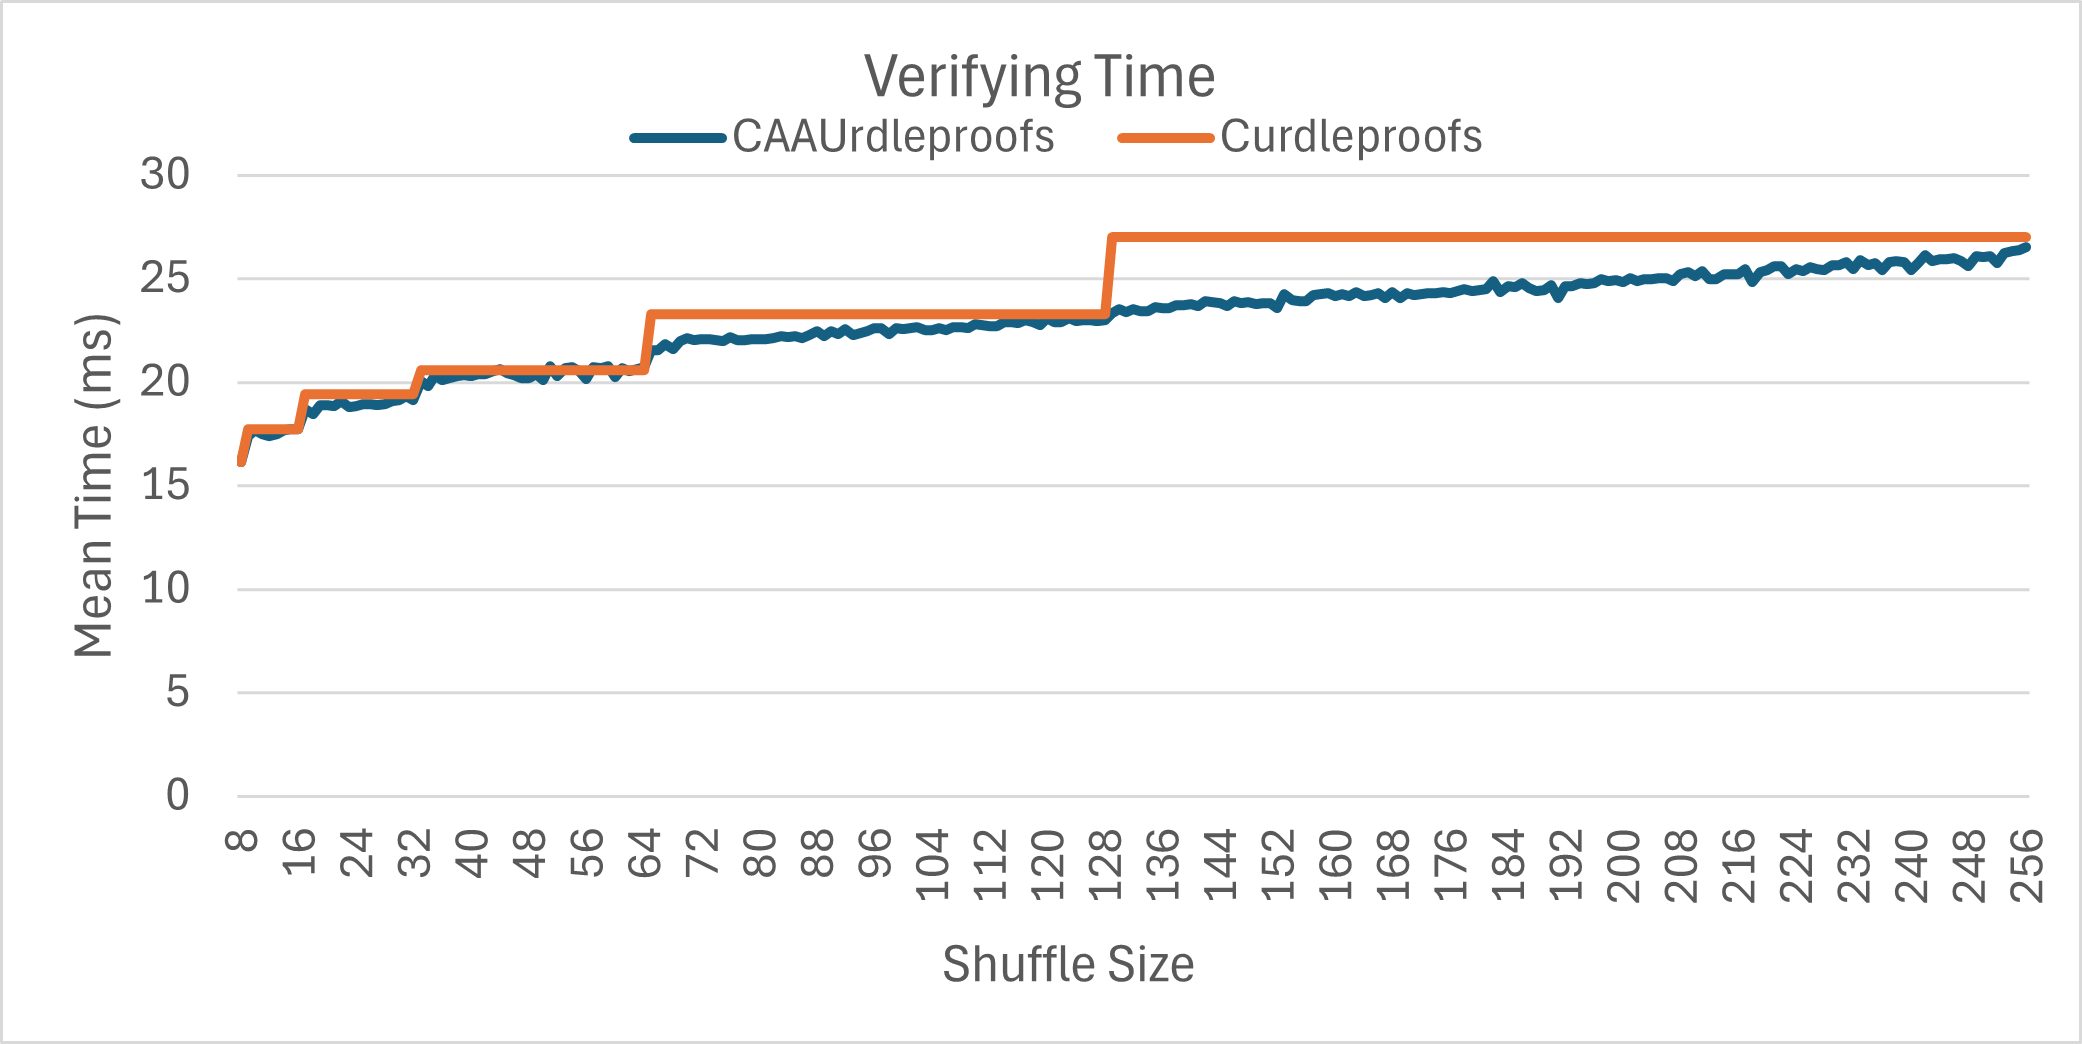
\includegraphics[width=0.45\textwidth]{figures/results/verifyingtime} }}%
    \caption{The timed results compared between CAAUrdleProofs and Curdleproofs}%
    \label{fig:resulttimes}%
\end{figure*}

After running the experiment where Curdleproofs and CAAUrdleproofs were compared across different shuffle sizes, we obtained the results shown in \autoref{fig:resulttimes}.

As mentioned in \autoref{sec:CAAUrdleproof-experiment}, CAAUdleproofs was run with a shuffle size $\ell$ of $\{8,9,\dots,256\}$ but Curdleproofs was only run with a shuffle size $\ell$ of $\{8,16,32,64,128,256\}$.
This is why the results for Curdleproofs show the shuffle size, $\ell$, instantly goes up to the next power of 2, because it theoretically would have to pad the input set until it reached the next power of 2.

From the results, we can see that CAAUrdleproofs and Curdleproofs have similar proving and verifying times when $\ell$ is a power of 2.
However, when $\ell$ is not a power of 2, CAAUrdleproofs is faster.

The results for the verifying time also shows that the verifying time jumps up the first four times it reaches a power of 2.

Additional to the proving and verifying times, the time used on shuffling is also lower for any $\ell$ that is not a power of 2.
Though, that was to be expected since CAAUrdleproofs uses the same shuffling algorithm as Curdleproofs but does not have to add additional padding values to the non power of 2 input sizes.



\subsection{Shuffle security}\label{subsec:Shuffle-security}

\begin{figure*}[!htb]
    \centering
    \subfloat[\centering]{{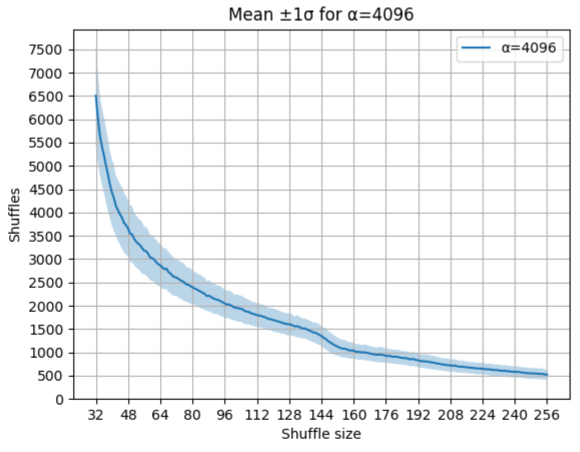
\includegraphics[width=0.45\textwidth]{figures/results/4096-256-p2} }}%
    \qquad
    \subfloat[\centering]{{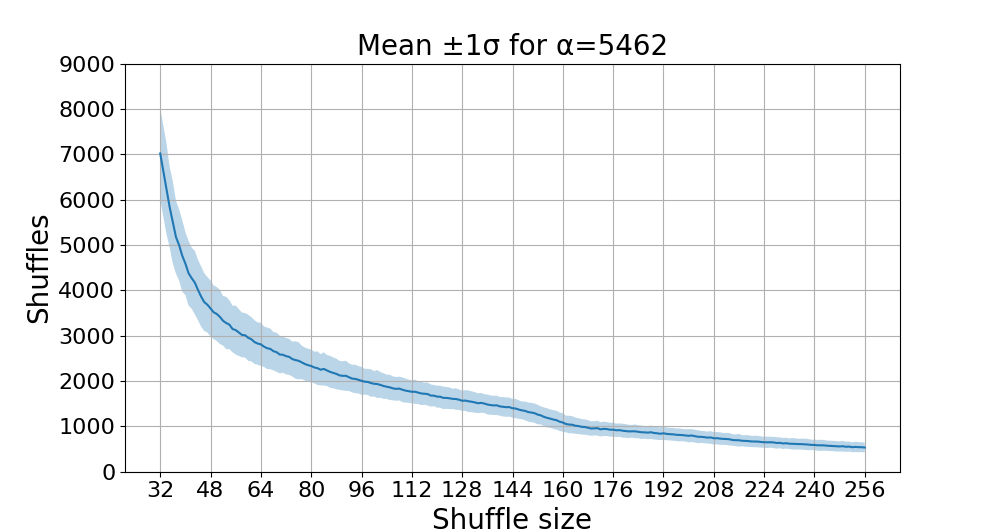
\includegraphics[width=0.45\textwidth]{figures/results/5462-256-p2} }}%
    \subfloat[\centering]{{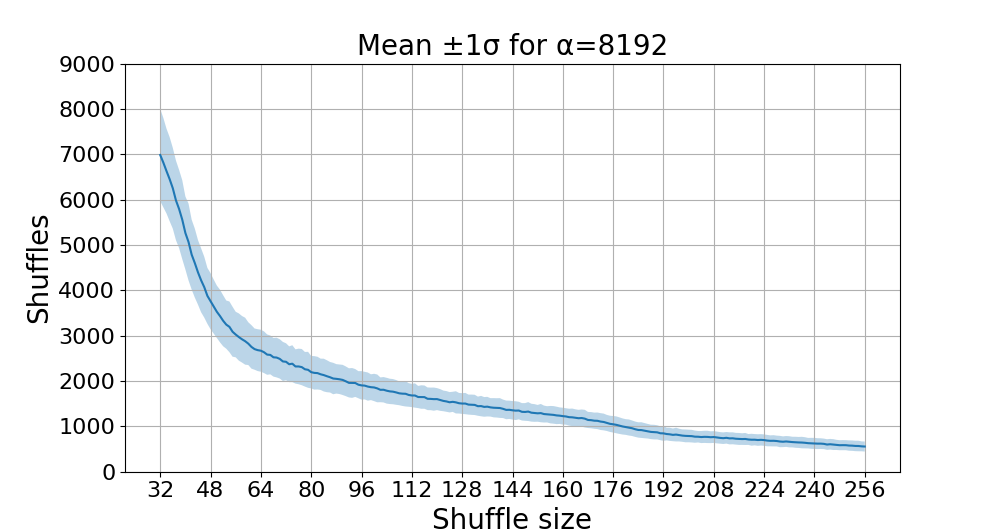
\includegraphics[width=0.45\textwidth]{figures/results/8192-256-p2} }}%
    \caption{The results of the shuffle security experiment showing the mean amount of honest shuffles necessary with one standard deviation}%
    \label{fig:shufflesecurity}%
\end{figure*}

The results of the shuffle security experiment are shown in \autoref{fig:shufflesecurity}.

\autoref{fig:shufflesecurity} shows the mean of the 1000 runs of each shuffle size $\ell$ as well as one standard deviation higher and lower.

We can see that the bigger the shuffle size $\ell$ is, the less honest shuffles are necessary to make the shuffle secure.
In Ethereum, each shuffling phase is limited to 8192 shuffles, meaning that the maximum number of honest shuffles that can be used is 8192.
Therefore, the results of the experiment also finds $T_H=T-\Beta$ being how many of the $T$ shuffles available durring the shuffling phase needing to be honest $T_H$ shuffles where the rest could then be the number of dishonest shuffles $\Beta$.
We also see that the bigger the shuffle size the narrower the standard deviation gets.

From the results of the experiment with $\alpha=8192$ we can see that number of honest shuffles necessary to make the shuffle secure sharply goes down until a size of $\ell=64$, and then it starts to flatten out.
we can see that with a size of $\ell=75$ we need about 1/3 of the shuffles to be honest to make the shuffle secure.
Likewise, we can see the at $\ell=108$ we need about 1/4 of the shuffles to be honest to make the shuffle secure.

In general all three of the experiments, despite the difference in $\alpha$, show the same trend.
They all level out but the higher the $\alpha$ is, the lower the leveling happens but the later it happens as well.
There are two things however that are different between the experiments.
At an $\alpha$ of 4096 we can see that at the start, with $\ell=32$, the mean number of honest shuffles necessary to make the shuffle secure is $\sim500$ lower than the 2 others.
As $\ell$ increases, the mean number of honest shuffles necessary to make the shuffle secure becomes similar to the other $\alpha$ values.
Another thing that differs between the experiments is that they all have sudden dip later on in the experiment.
Here we can see a trend that the lower the~$\alpha$ is, the earlier the dip happens.

\begin{figure*}[!htb]
    \centering
    \subfloat[\centering]{{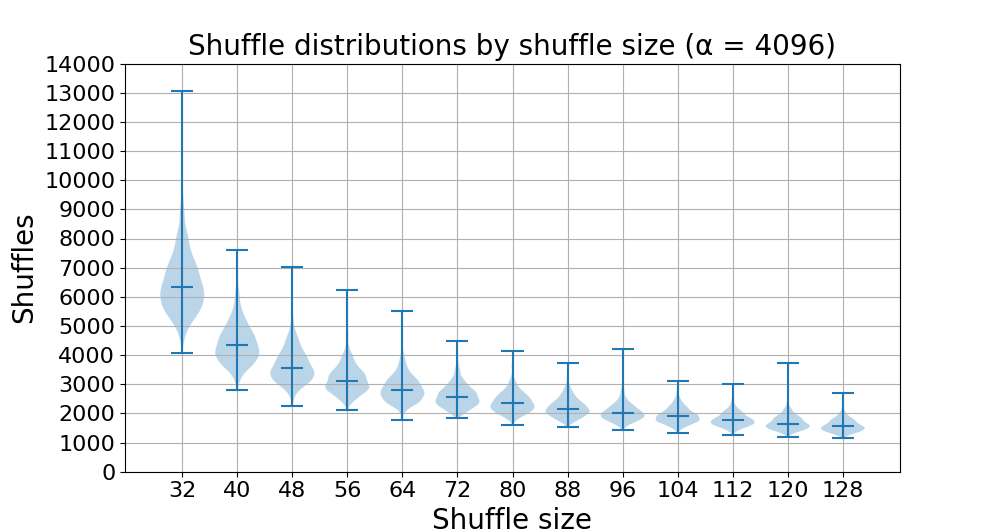
\includegraphics[width=0.45\textwidth]{figures/results/violin-4096} }}%
    \qquad
    \subfloat[\centering]{{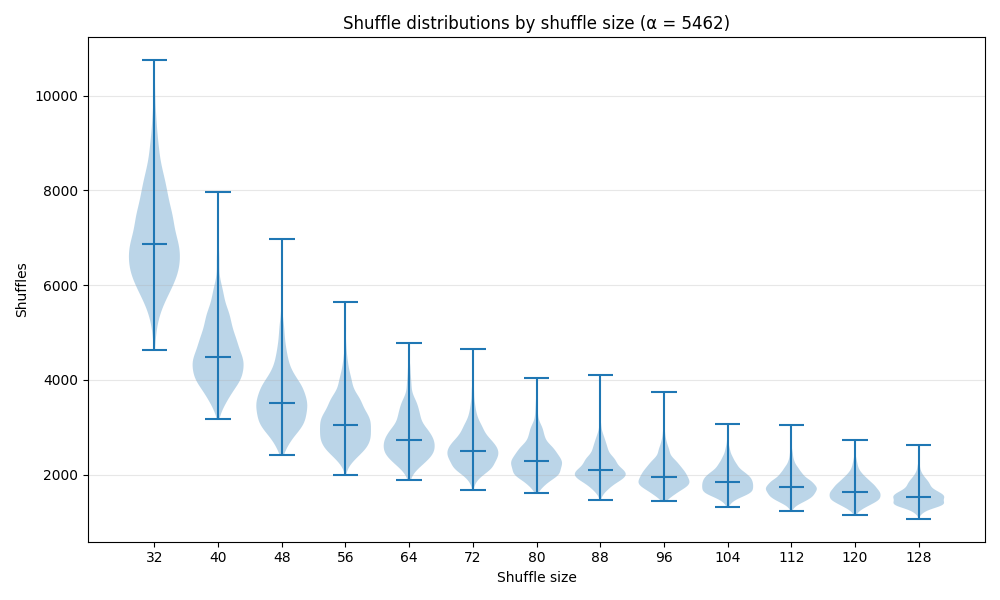
\includegraphics[width=0.45\textwidth]{figures/results/violin-5462} }}%
    \subfloat[\centering]{{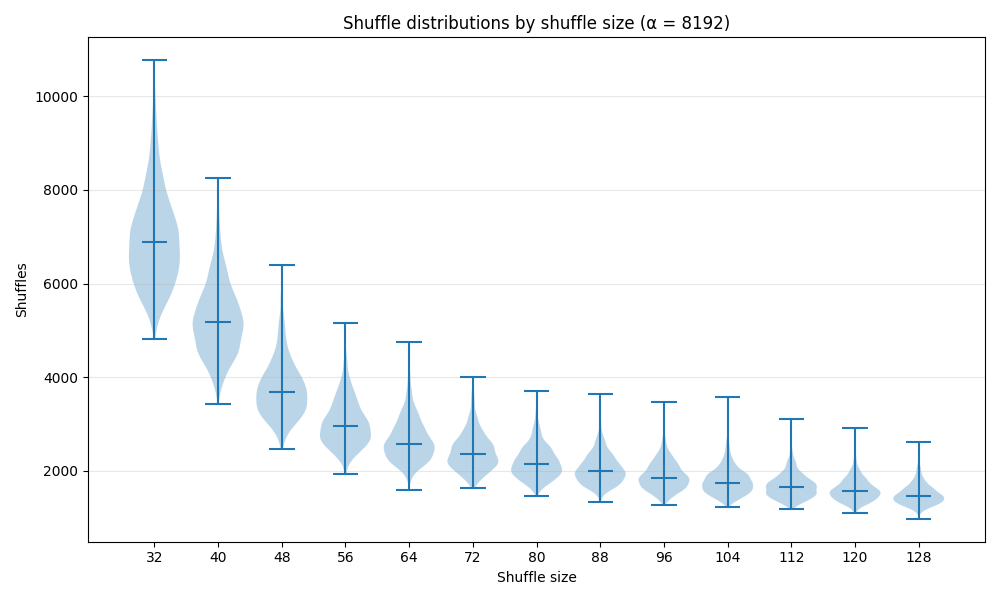
\includegraphics[width=0.45\textwidth]{figures/results/violin-8192} }}%
    \caption{The results of the shuffle security experiment showing the spread of nessecary shuffle need for the shuffle to be secure}%
    \label{fig:shufflesecurityviolin}%
\end{figure*}

The results in \autoref{fig:shufflesecurityviolin} show that for all three $\alpha$ values, the spread of the necessary honest shuffles tightens the larger the shuffle size $\ell$ gets.
Like the results in \autoref{fig:shufflesecurity}, \autoref{fig:shufflesecurityviolin} also shows that the bigger a shuffle size $\ell$, the less honest shuffles on average are necessary to make the shuffle secure.

It is worth noting that there is a spike in the distribution of the necessary honest shuffles at $\ell=32$ for $\alpha=4096$.
This spike is not present for the other two $\alpha$ values, and is due to the probabilistic nature of the shuffling method.

Another thing that is notable is that in the setting of Ethereum, the maximum number of shuffles available is 8192.
This means that in the cases where more than the 8192 shuffles where necessary to make the shuffle secure, the shuffle would not have been secure within the Ethereum setting.
Therefore, it is also possible to see the experiment as running 1000 days worth of each shuffle size $\ell$ and then seeing how many of those days would have been secure.
This means that the first size of $\ell$ that could have been secure for the entire durration of the experiment would be $\ell=42$ for $\alpha=8192$ and $\ell=40$ for $\alpha=5462$ and $\alpha=4096$.


